\subsection{Client Interface}

After login, the \aclient[] is greeted with the \textit{main} screen, wich gives three posebilities:
\begin{itemize}
	\item Add problem
	\item My problems
	\item Search for problem(s)
\end{itemize}

\paragraph{Add problem} as the name dictates, initiates the process of adding a specific problem to \hdesk[].
\paragraph{My problems}
\paragraph{Search for problem(s)}



\begin{figure}[h]
\begin{center}
 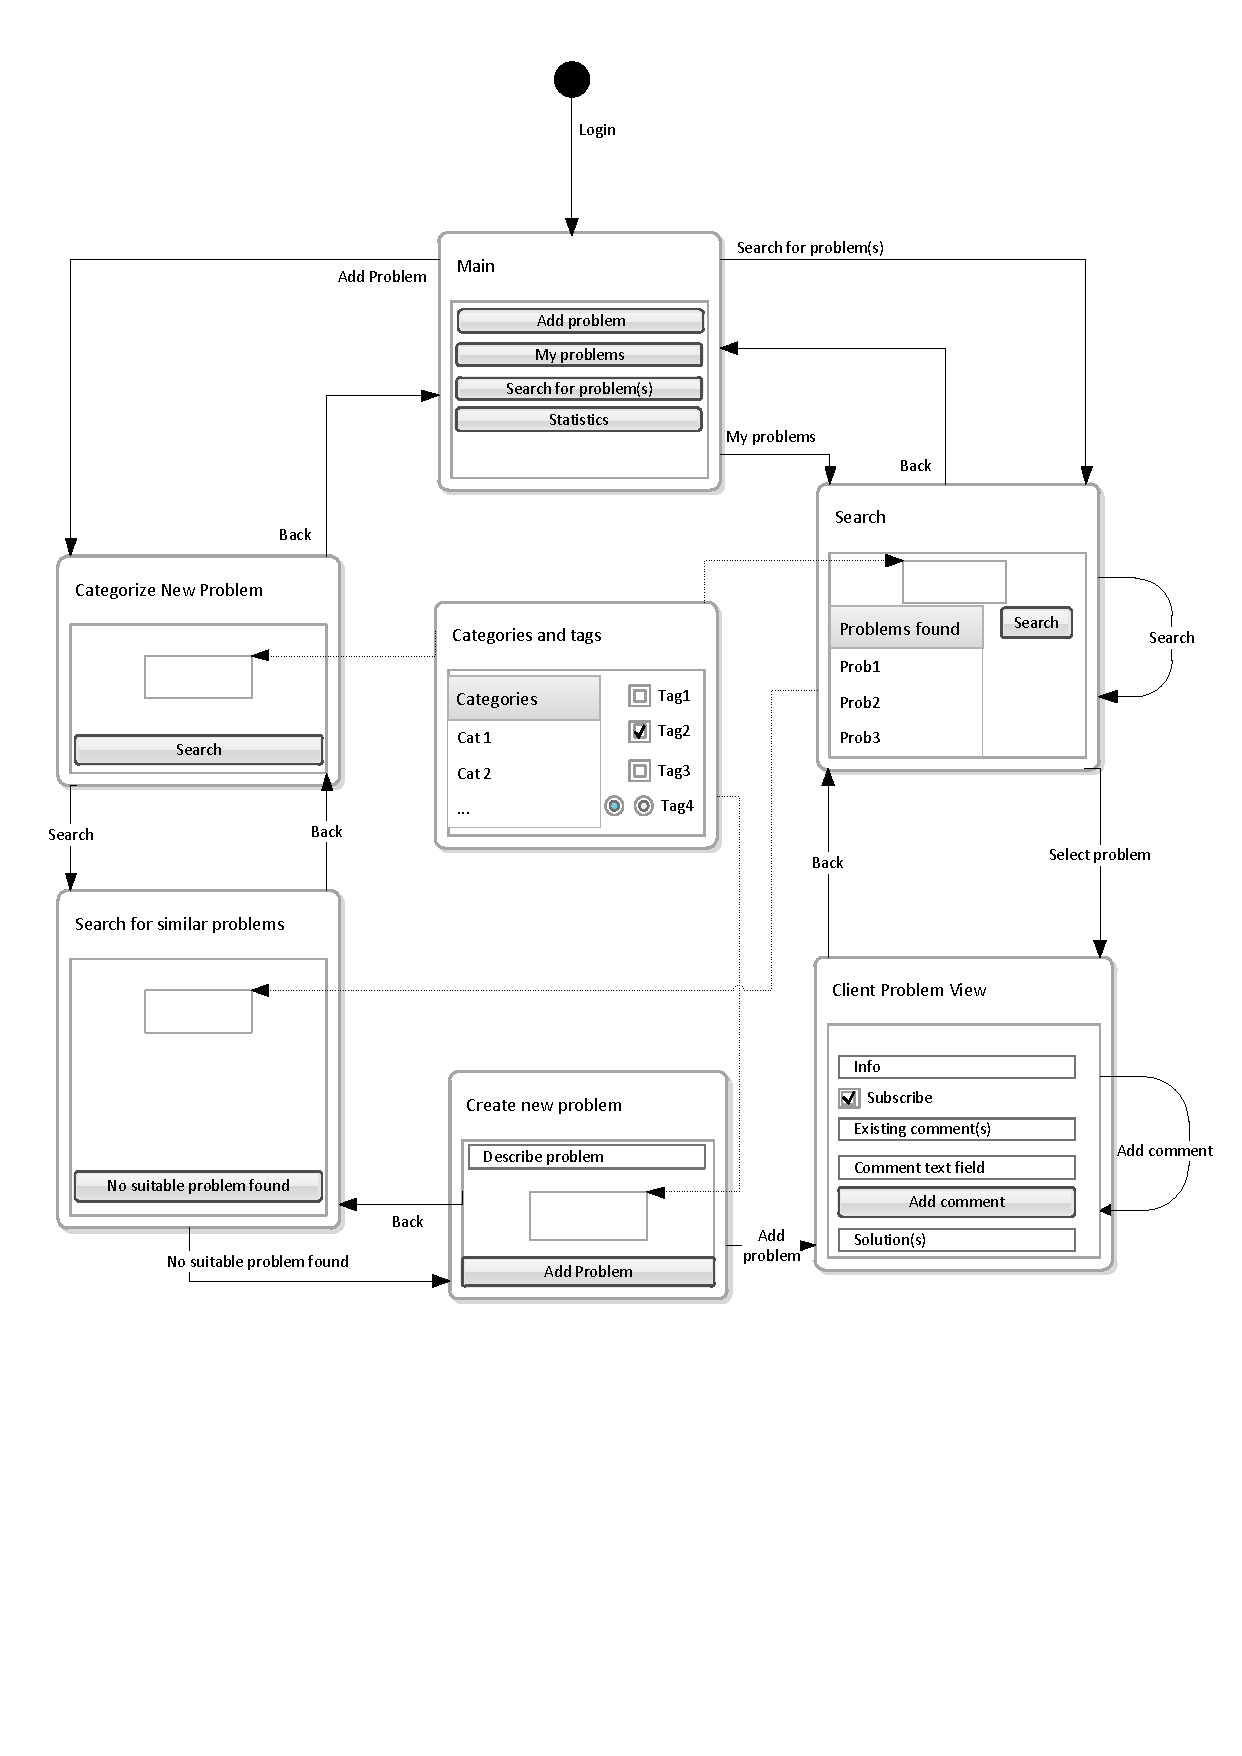
\includegraphics[scale=0.70]{input/application_domain_analysis/client_interface}
\caption{\Client[] interface}
\label{fig:client_interface}
\end{center}
\end{figure}

